\section*{\centering Annexes}
\vspace*{30px}

\begin{enumerate}
	\item \textbf{annexe1} : Organigramme fonctionnel de l'académie de Rennes.\\
	\item \textbf{annexe2} : Organigramme du service informatique académique de Rennes (DSII).\\
	\item \textbf{annexe3} : Exemple du fichier User de la plateforme d'authentification Keycloak
\end{enumerate}

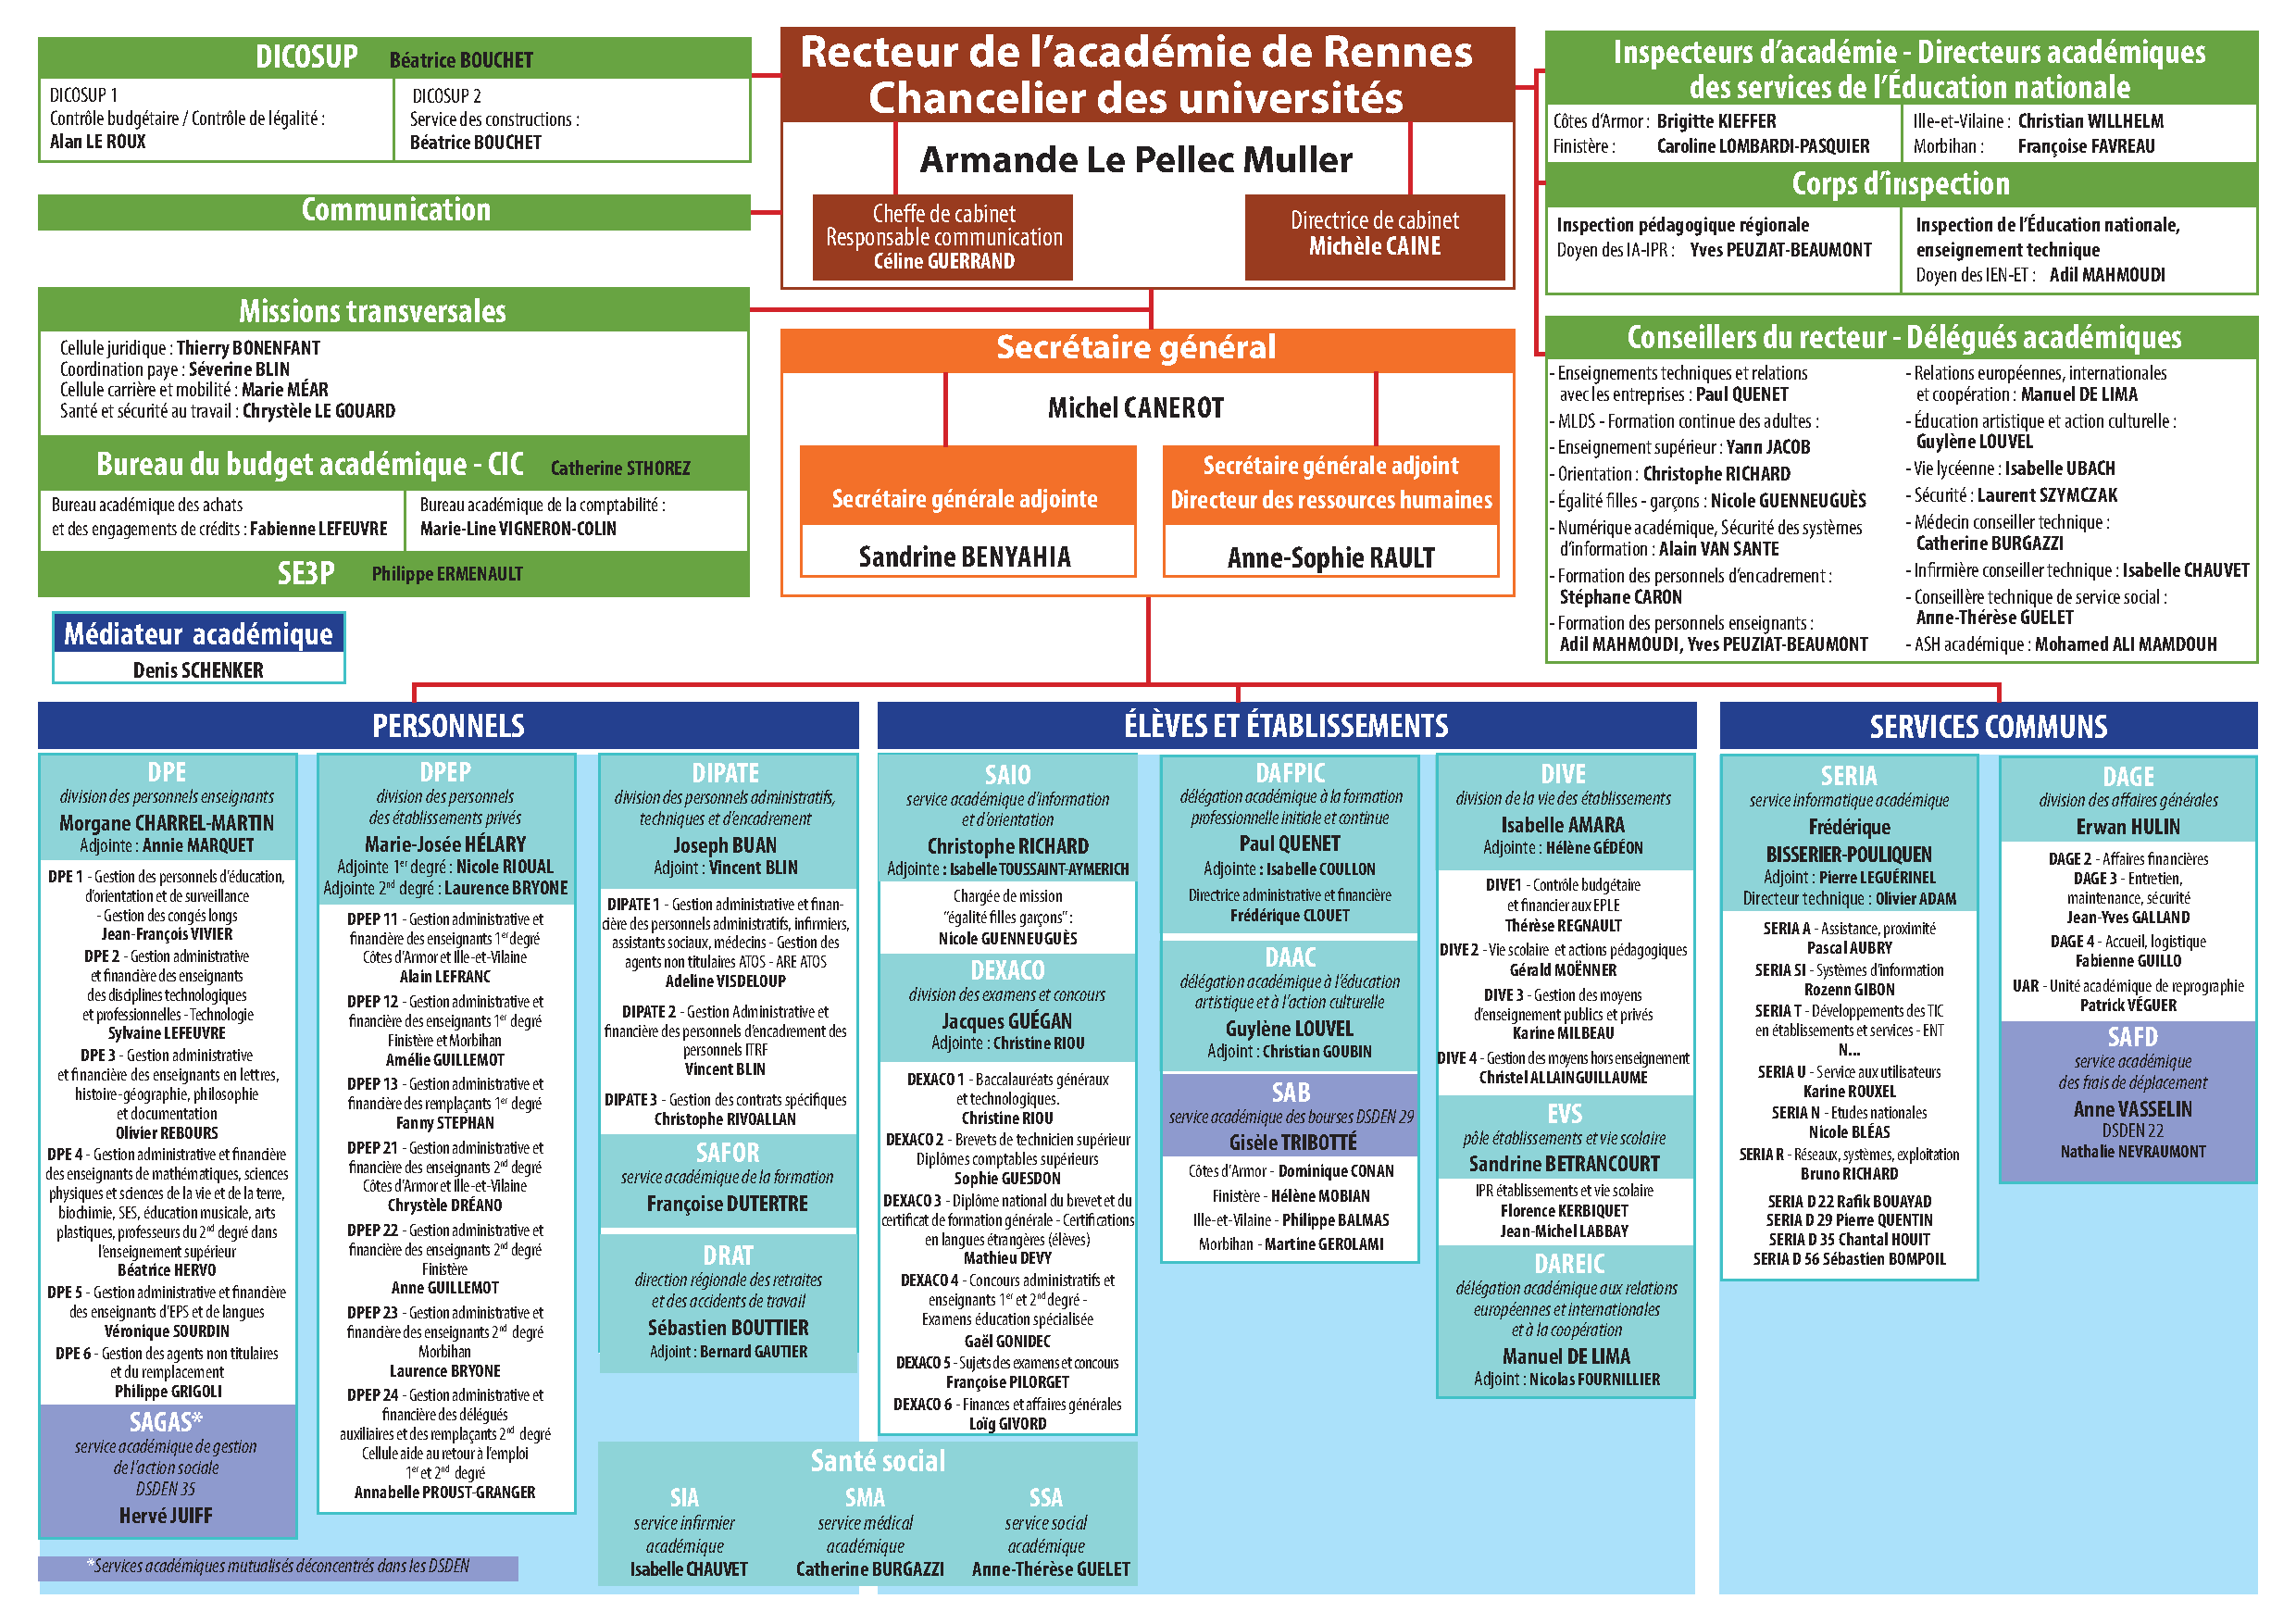
\includepdf[angle=90]{./pdf/ac_rennes.pdf}
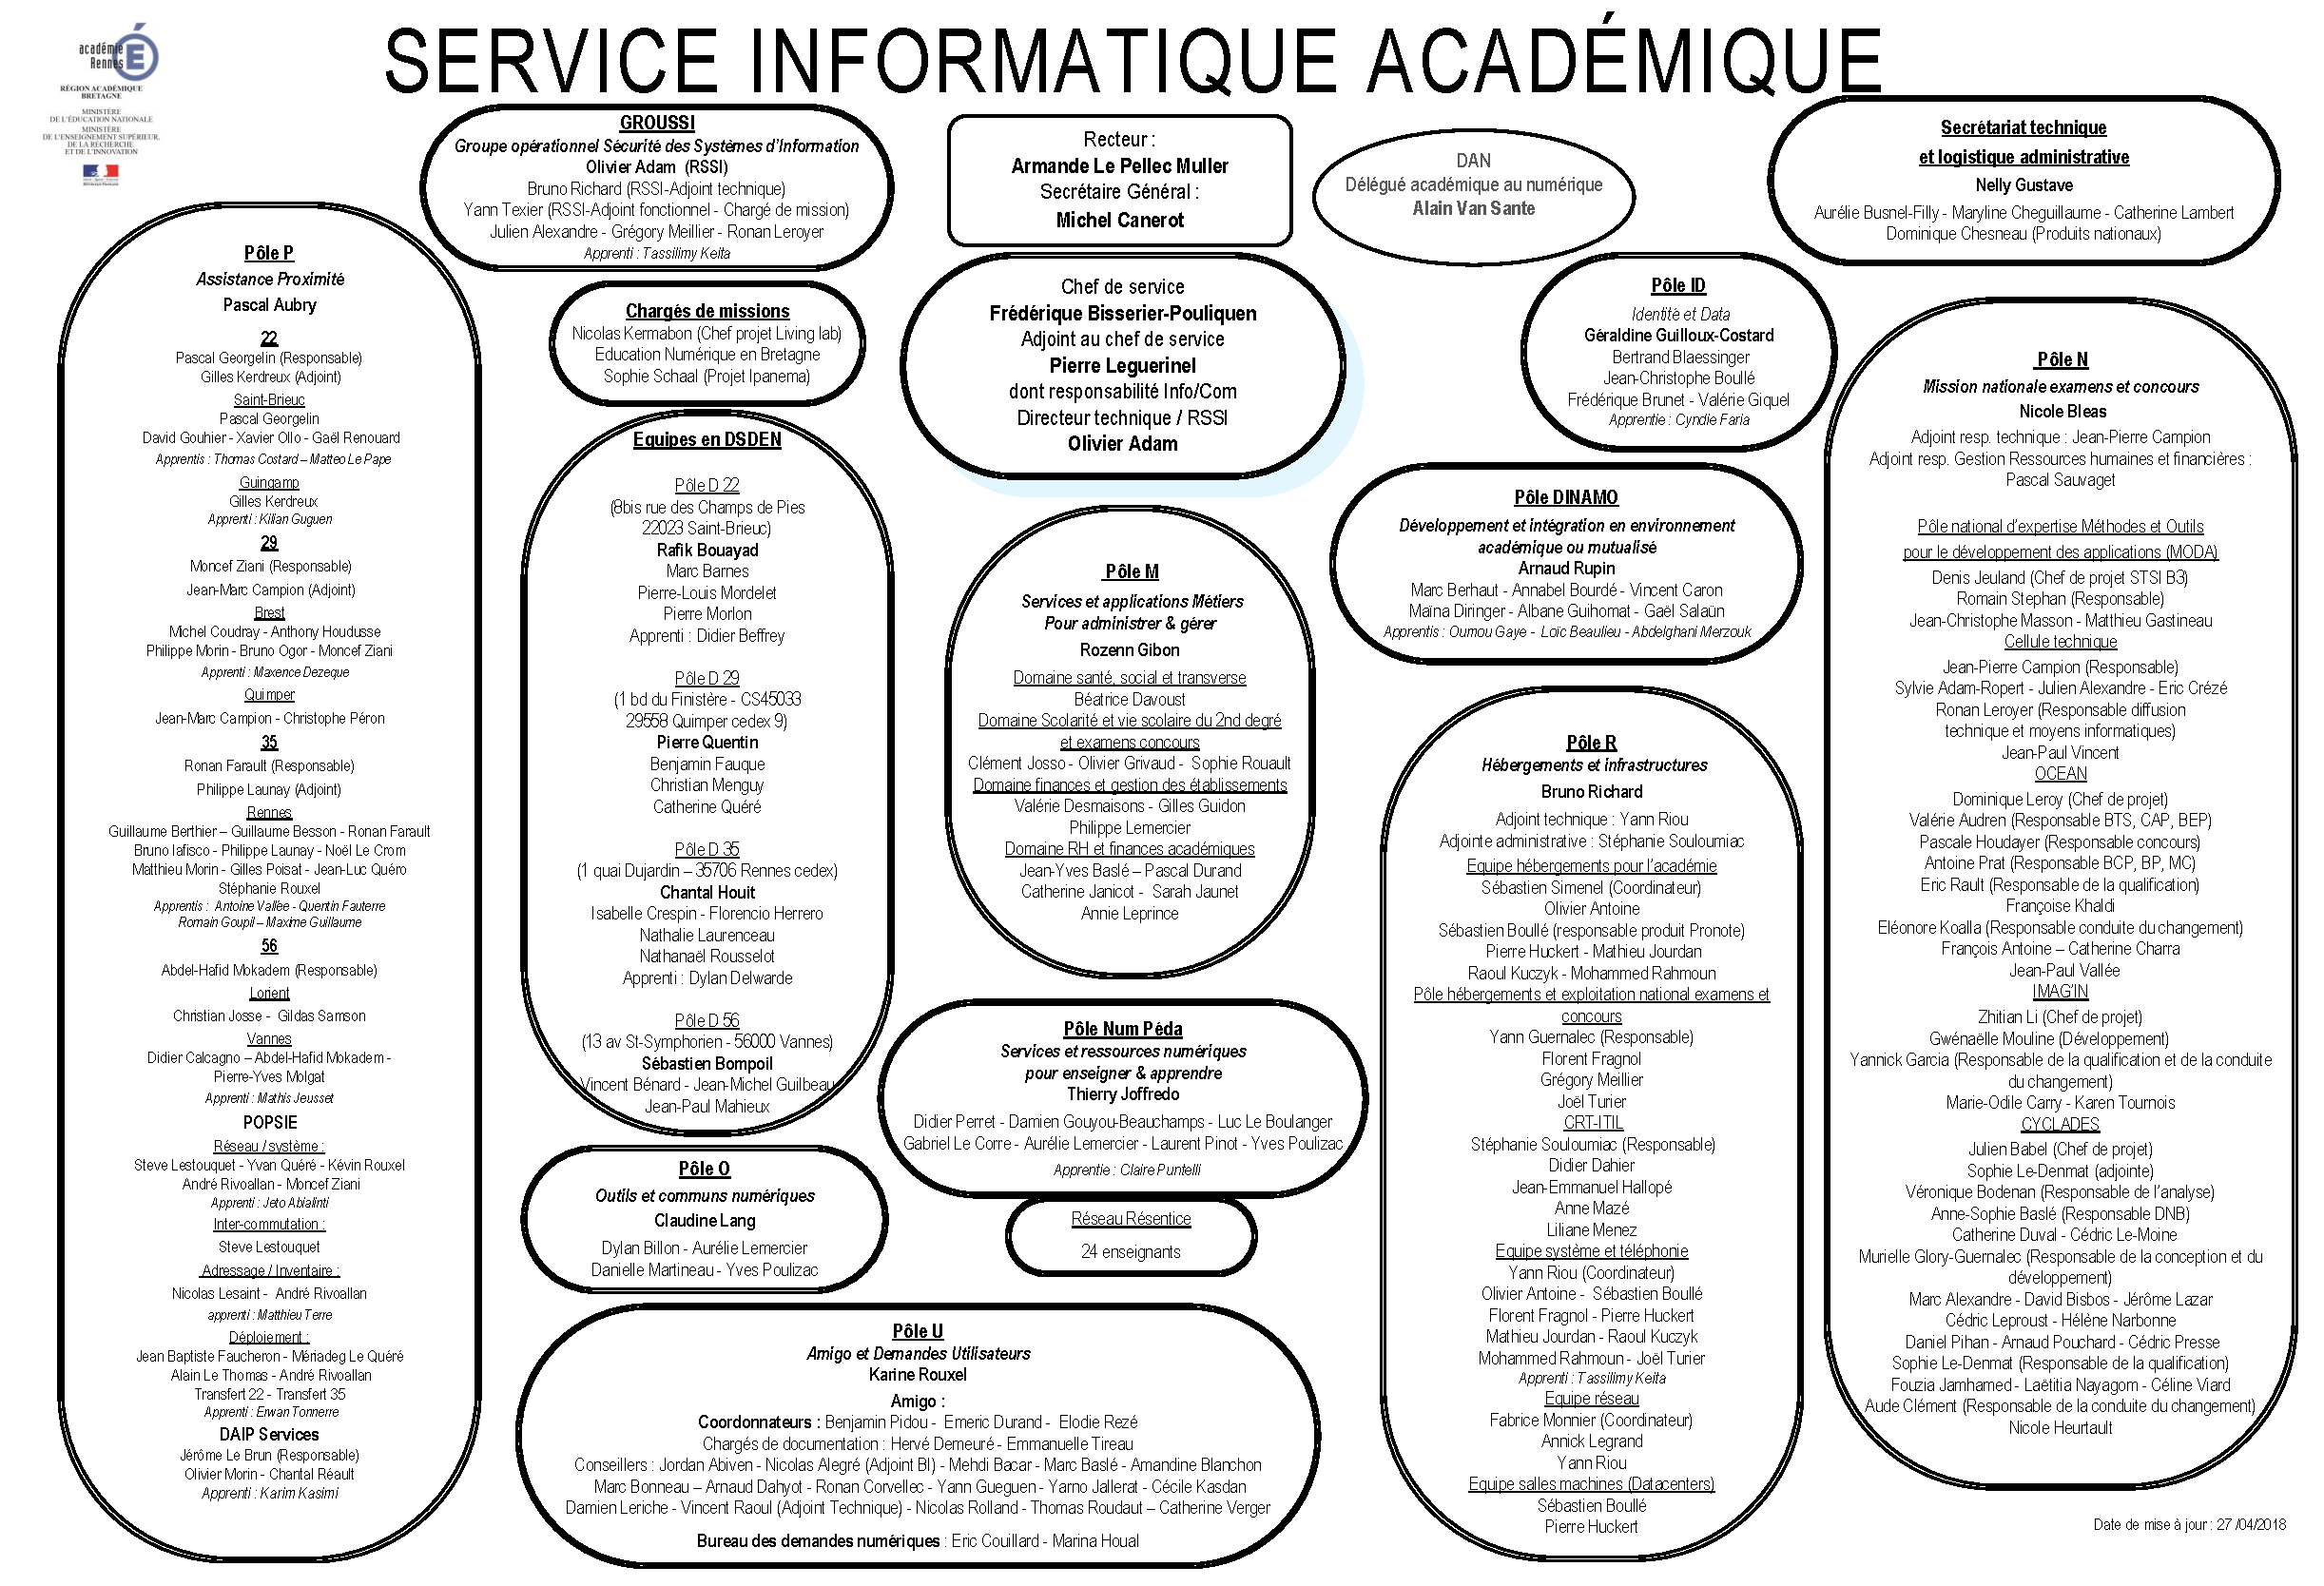
\includepdf[angle=90]{./pdf/orgSeria.pdf}
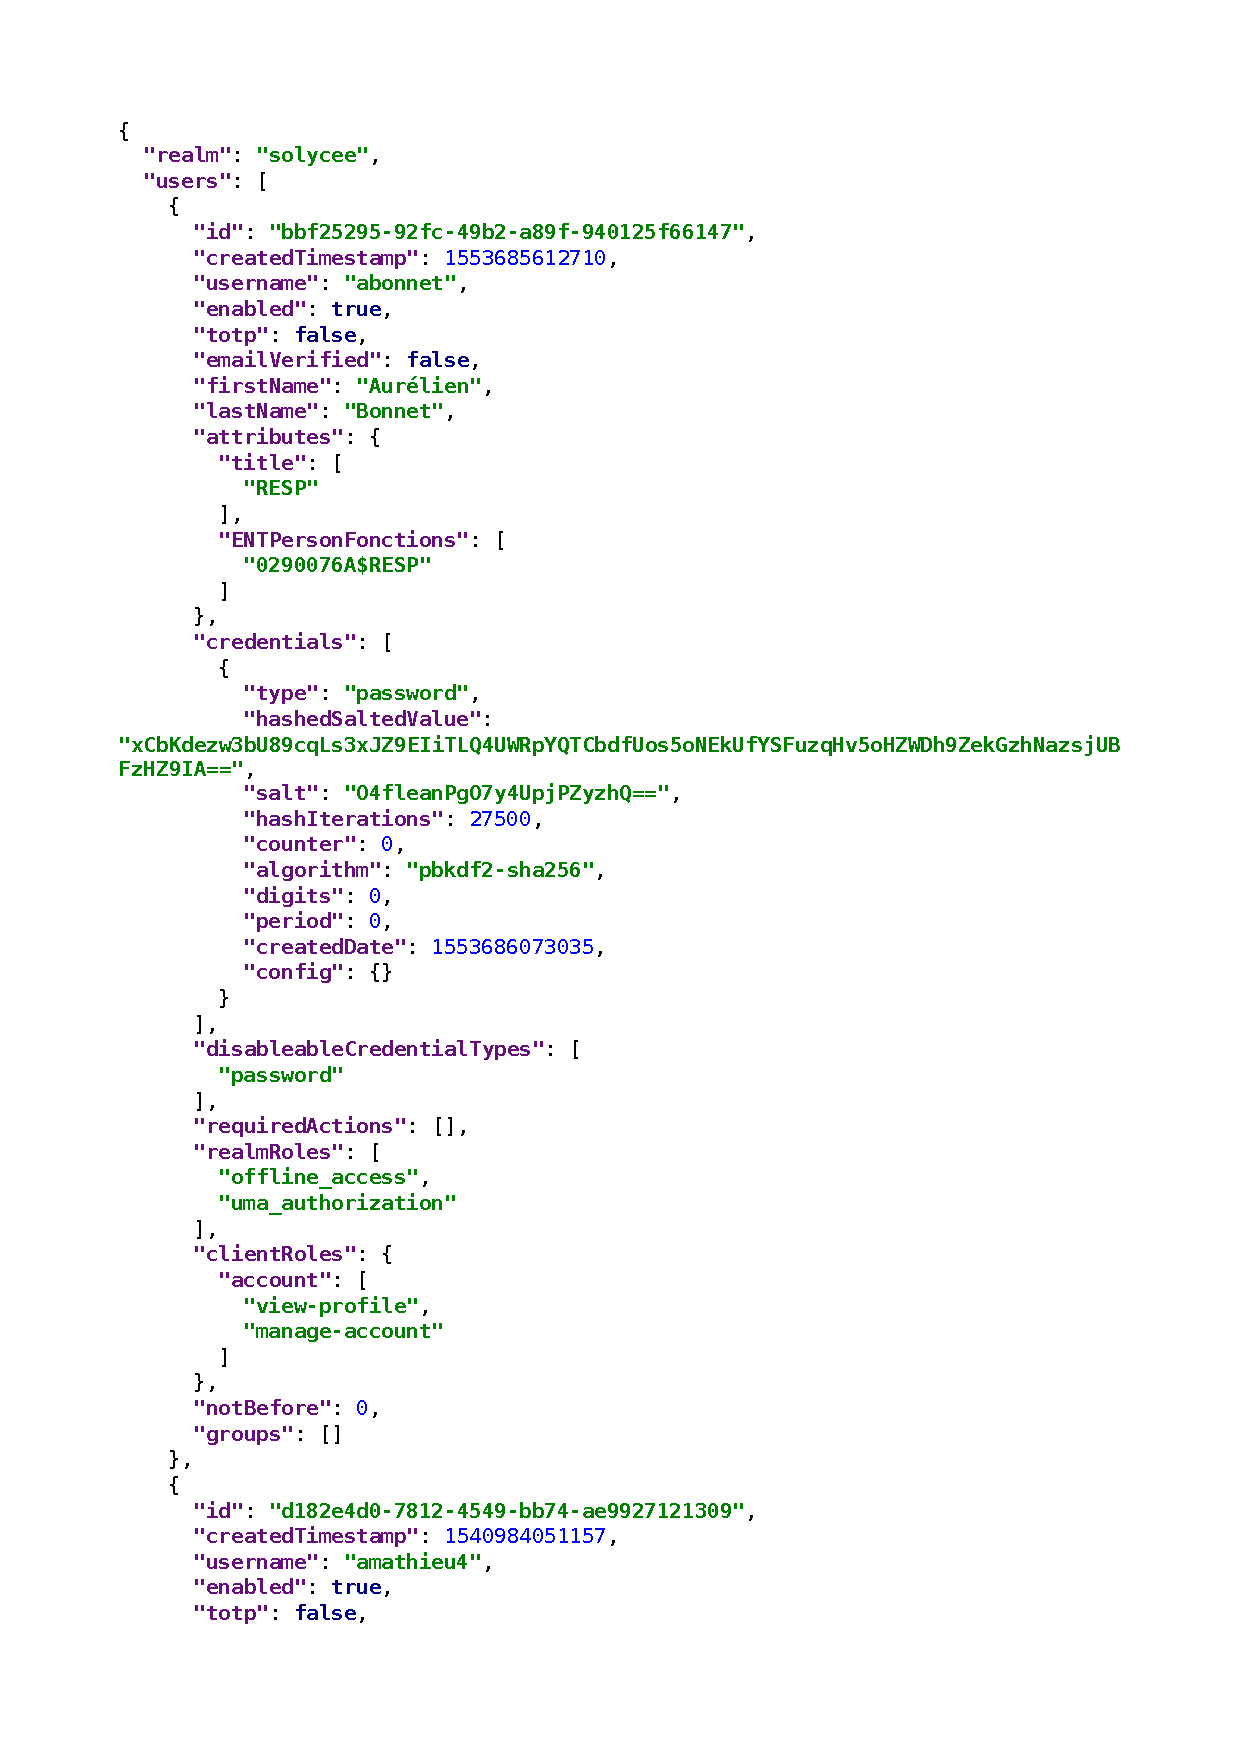
\includepdf{./pdf/Keycloak-users.pdf}

\begin{figure}[H]
	\centering
 		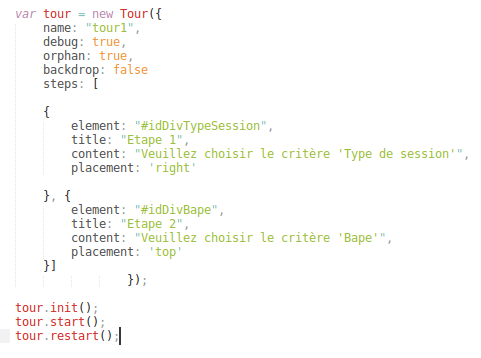
\includegraphics[width=1\textwidth]{pdf/bootstrap_tour.png}
  		\caption{Exemple de Bootstrap Tour }
 \end{figure}
 
 
 \begin{figure}[H]
	\centering
 		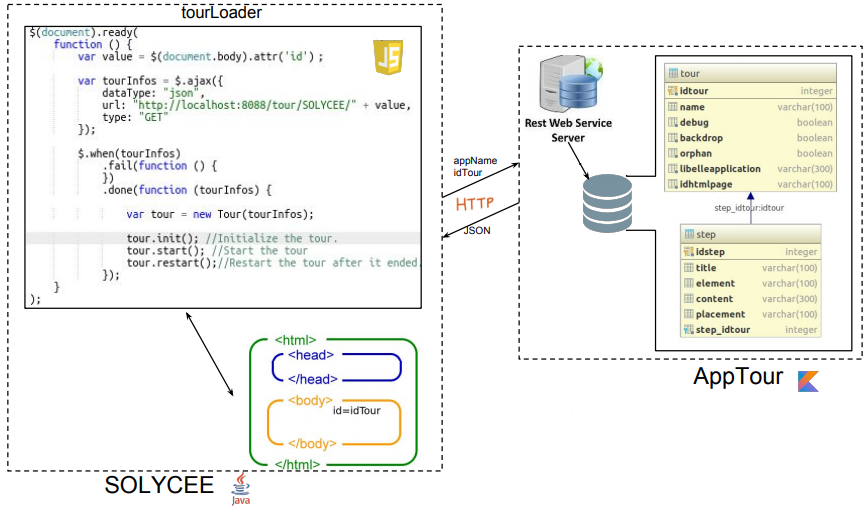
\includegraphics[width=1\textwidth]{pdf/architecture.png}
  		\caption{Architecture de la version 2 avec AppTour }
 \end{figure}

\vfill

\vfill

\addcontentsline{toc}{chapter}{Annexes}


